\documentclass{beamer}

\usepackage{lads}
\setbeamertemplate{navigation symbols}{}

\title{Linear Models}
\date{}
\author{BIOE 210}

\begin{document}

\maketitle

\begin{frame}
\frametitle{A simple linear system}

Let's solve the linear system
\[ y = \beta x \]
When $y=2.4$ and $x=2$. What is the value of $\beta$?

\pause
\[ \beta = y/x = 2.4/2 = 1.2 \]
\end{frame}

\begin{frame}
\frametitle{A \emph{noisy} linear system}

\begin{columns}
\begin{column}{0.3\textwidth}
\begin{center}
  \begin{tabular}{cccc}
    \toprule
    \xobs & \yobs \\
    \midrule
    0.07 & -0.05 \\
    0.16 & 0.40 \\
    0.48 & 0.66 \\
    0.68 & 0.65 \\
    0.83 & 1.12 \\
    \bottomrule
  \end{tabular}
\end{center}	
\end{column}

\begin{column}{0.7\textwidth}
\begin{center}
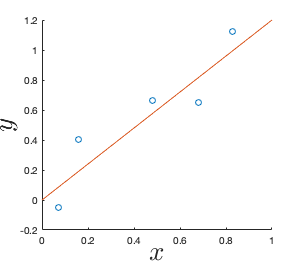
\includegraphics{simple_lin_scatter.png}
\end{center}	
\end{column}
\end{columns}
	
\end{frame}


\begin{frame}
\frametitle{Each point gives a bad estimate of $\beta$}

\begin{columns}
\begin{column}{0.3\textwidth}
\begin{center}
  \begin{tabular}{cccc}
    \toprule
    \xobs & \yobs \\
    \midrule
    0.07 & -0.05 \\
    0.16 & 0.40 \\
    0.48 & 0.66 \\
    0.68 & 0.65 \\
    0.83 & 1.12 \\
    \bottomrule
  \end{tabular}
\end{center}	
\end{column}

\begin{column}{0.7\textwidth}
\begin{align*}
	1.&\quad \beta = -0.05/0.07 = -0.7 \\
	2.&\quad \beta = 0.40/0.16 = 2.5  \\
	3.&\quad \beta = 0.66/0.48 = 1.3 \\
	4.&\quad \beta = 0.65/0.68 = 0.9 \\
	5.&\quad \beta = 1.12/0.83 = 1.3
\end{align*}
\end{column}
\end{columns}

\pause
\begin{center}
Average $\beta = 1.09$, not the true value of 1.2.

Using \emph{linear regression} we can use the same data to estimate $\beta = 1.21$.
\end{center}

\end{frame}

\begin{frame}
\frametitle{Quantifying Error}
The goal of linear regression is to minimize the error between the model and the observed data.

\pause
\bigskip
Error has two properties:
\begin{enumerate}
	\item $\error{\yobs,\ypred} \ge 0$
	\item $ \error{\yobs,\ypred} = 0 \iff \yobs = \ypred $
\end{enumerate}

\pause
\bigskip
There are many ways to define error:
\begin{enumerate}
	\item $\error{\yobs,\ypred} = |\yobs - \ypred |$
	\item $\error{\yobs,\ypred} = (\yobs - \ypred)^2$
\end{enumerate}
\end{frame}


\begin{frame}
\frametitle{Why choose the squared error?}
\begin{itemize}
	\item Quadratic functions are continuously differentiable.
	\item The squared error fights against outliers.
	\item Minimizing squared error has a unique solution.
\end{itemize}
\end{frame}

\begin{frame}
\frametitle{Fitting Linear Models}
\begin{enumerate}
	\item Choose a model that you think explains the relationship between inputs ($x$) and outputs ($y$). The models should contains unknown parameters ($\beta$) that you will fit to a set of observations.
	\item Find values for $\beta$ by minimizing the total error between the observed outputs (\yobs) and the outputs predicted from the model
	\[ \min_{\beta} \sum_{\yobs}\left(\yobs - \ypred\right)^2 \]
Substitute the model you selected in Step 1 in place of \ypred\ in the above minimization.
	\item Minimize the function by taking the derivative of the sum squared error and setting it equal to zero. Solve for the unknown parameters $\beta$.
\end{enumerate}	
\end{frame}

\begin{frame}
\frametitle{Fitting a single parameter linear model}
The simplest linear model has only a single parameter
\[ \ypred = \beta_0 \]

\pause
Assume we have $n$ observations ($\xobs,\yobs$). The total error is
\[ \min_{\beta_0} \sum_{i=1}^n \left(\yobs_i - \ypred_i\right)^2 \]
\pause
Substituting our model we have
\[ \min_{\beta_0} \sum_{i=1}^n \left(\yobs_i - \beta_0\right)^2 \]
\end{frame}

\begin{frame}
\frametitle{Solving for the unknown parameter $\beta_0$}
\begin{align*}
	\frac{d}{d\beta_0}\left(\sum_{i=1}^n(\yobs_i-\beta_0)^2\right) & = 0 \\
	\sum_{i=1}^n \left(\frac{d}{d\beta_0}(\yobs_i-\beta_0)^2\right) & = 0 \\
	\sum_{i=1}^n \left( 2(\yobs_i-\beta_0)(-1) \right) & = 0 \\
	-2\sum_{i=1}^n(\yobs_i-\beta_0) & = 0 \\
	\sum_{i=1}^n\yobs_i - \sum_{i=1}^n\beta_0 &= 0 \\
	\sum_{i=1}^n\yobs_i - n\beta_0 &= 0 \\
\end{align*}	
\end{frame}

\begin{frame}
\frametitle{Final solution for the single parameter model}
For the simple linear model
\[ \ypred = \beta_0 \]

the least-squares estimate of the parameter $\beta_0$ is
\[ 	\beta_0 = \frac{1}{n}\sum_{i=1}^n\yobs_i \]

\pause
This is the mean! So that's where the mean comes from.
\end{frame}

\begin{frame}
\frametitle{The two parameter linear model}
The next simplest model has two unknown parameters
\[ \ypred = \beta_0 + \beta_1 x \]

\pause
How much more work does it take to fit this model?
\bigskip
Stop the video and work through \S 14.2.
\end{frame}

\begin{frame}
\frametitle{Well, that got out of hand quickly.}

We can derive estimates for any type of linear model. But the amount of math scales cubicly with the number of parameters (why?).

\bigskip
Instead, let's turn to a matrix formalism for linear models.	
\end{frame}

\begin{frame}
\frametitle{A matrix formalism for linear models}
Let's write out one equation for each observation of the model $y = \beta_0 + \beta_1x$.
\begin{align*}
	-0.05 = \beta_0 + 0.07\beta_1 + \epsilon_1 \\
	0.40 = \beta_0 + 0.16\beta_1 + \epsilon_2 \\
	0.66 = \beta_0 + 0.48\beta_1 + \epsilon_3 \\
	0.65 = \beta_0 + 0.68\beta_1 + \epsilon_4 \\
	1.12 = \beta_0 + 0.83\beta_1 + \epsilon_5
\end{align*}

\pause
\[ \begin{pmatrix} -0.05\\ \phan0.40\\ \phan0.66\\ \phan0.65\\ \phan1.12 \end{pmatrix} = \begin{pmatrix} 1&0.07\\ 1&0.16\\ 1&0.48\\ 1&0.68\\ 1&0.83 \end{pmatrix} \vectwo{\beta_0}{\beta_1} + \begin{pmatrix} \epsilon_1\\ \epsilon_2\\ \epsilon_3\\ \epsilon_4\\ \epsilon_5 \end{pmatrix} \]
\pause
\[ \Vy = \V{X}\Vbeta+\Vepsilon \]	
\end{frame}

\begin{frame}
\frametitle{Solving the linear system}

A few points about $\Vy = \V{X}\Vbeta+\Vepsilon$:
\begin{itemize}
	\item The unknowns are \Vbeta, not \V{X}.
	\item The coefficient matrix \V{X}\ is called the \emph{design matrix}.
	\item The design matrix \V{X}\ is rarely square.
\end{itemize}

\pause
The solution to this system that minimizes the errors in \Vepsilon\ is 
\[ \Vbeta = \VX^+\Vy \]
where $\VX^+$ is the \emph{pseudoinverse} of \VX.
\end{frame}

\begin{frame}
\frametitle{For next time}
\begin{itemize}
	\item Follow through the end of Chapter 14 to see how we calculate and use the pseudoinverse.
	\item Next time we will demonstrate how to formulate and solve more complex linear models.
\end{itemize}	
\end{frame}

\begin{frame}
\frametitle{What is an interaction?}	

Imagine we're modeling the response ($y$) from two input variables, $x_1$ and $x_2$. The simplest model is

\[ y = \beta_1x_1 + \beta_2x_2 + \epsilon \]

\pause
The coefficient $\beta_1$ measures the effect of $x_1$ and $\beta_2$ measures the effect of $x_2$. These effects are \textbf{independent}.

\bigskip
\pause
What is there is another effect that depends on both $x_1$ and $x_2$? This is an \textbf{interaction} between $x_1$ and $x_2$.
\end{frame}

\begin{frame}
\frametitle{How do we model interactions?}

We model the interaction of $x_1$ and $x_2$ using the product of these variables.
\[ y = \beta_1x_1 + \beta_2x_2 + \beta_{12}x_1x_2 + \epsilon \]

The coefficient $\beta_{12}$ is the effect size of the interaction.

\pause
\bigskip
Why do we multiply $x_1$ and $x_2$? There are at least two ways to interpret this term.
\end{frame}

\begin{frame}
\frametitle{The coded factor interpretation}

Often we set up design matrices using \textbf{coded variables}. If we're testing the variable at two levels, we code the variable as ``on/off"~($\{0,1\}$) or ``low/high"~($\{-1,+1\}$).

\pause
\bigskip
\begin{columns}
\begin{column}{0.55\textwidth}
on/off $\rightarrow$ interaction when both ``on"
\begin{center}
\begin{tabular}{cc|c}
	$x_1$ & $x_2$ & $x_1x_2$ \\
	\hline
	0 & 0 & 0 \\
	0 & 1 & 0 \\
	1 & 0 & 0 \\
	1 & 1 & 1
\end{tabular}
\end{center}
\end{column}

\pause
\begin{column}{0.5\textwidth}
high/low $\rightarrow$ interaction when both ``high" or both ``low"
\begin{center}
\begin{tabular}{cc|c}
	$x_1$ & $x_2$ & $x_1x_2$ \\
	\hline
	$-1$ & $-1$ & $+1$ \\
	$-1$ & $+1$ & $-1$ \\
	$+1$ & $-1$ & $-1$ \\
	$+1$ & $+1$ & $+1$
\end{tabular}
\end{center}
\end{column}
\end{columns}

\end{frame}

\begin{frame}
\frametitle{The augmented slope interpretation}

We can also interpret the interaction as one variable changing the effect of the other variable.

\begin{align*}
	y &= \beta_1x_1 + \beta_2(x_1)x_2 + \epsilon \\
	 &= \beta_1x_1 + (\beta_2 + \beta_{12}x_1)x_2 + \epsilon \\
	 &= \beta_1x_1 + \beta_2x_2 + \beta_{12}x_1x_2 + \epsilon
\end{align*}
\end{frame}

\begin{frame}
\frametitle{Things to remember about interactions}

\begin{itemize}
	\item Interaction are modeled as the product of variables.
	\item The interaction effect is ``above and beyond" the independent effects (synergy/super-additivity, antagonism/sub-additivity).
	\item Higher-order interactions are possible (e.g. $x_1x_2x_3$), but these are rare.
\end{itemize}
\end{frame}


\end{document}
